\documentclass[12pt]{article}
\usepackage{light}

\hidesolutions
%\showsolutions

\newcommand{\edge}[2]{#1\text{---}#2}
\newcommand{\mfigure}[3]{\bigskip\centerline{\resizebox{#1}{#2}{\includegraphics{#3}}}\bigskip}

\begin{document}

\recitation{8}{October 3, 2014}

%%%%%%%%%%%%%%%%%%%%%%%%%%%%%%%%%%%%%%%%%%%%%%%%%%%%%%%%%%%%%%%%%%%%%%%%%%%%%%%
\section*{Routing in a Bene\u{s} Network}

In lecture, we saw that the Bene\u{s} network has a max congestion of
1; that is, every permutation can be routed in such a way that a
single packet passes through each switch.  Let's work through an
example.  A Bene\u{s} network of size $N = 8$ is attached.

\begin{enumerate}
\item Within the Bene\u{s} network of size $N = 8$, there are two
subnetworks of size $N = 4$.  Put boxes around these.  Hereafter,
we'll refer to these as the \textit{upper} and \textit{lower}
subnetworks.

\solution{
\ \\
\mfigure{!}{2in}{benes-decomp}
}

\item Now consider the following permutation routing problem:
%
\begin{align*}
\pi(0) & = 3 & \pi(4) & = 2 \\
\pi(1) & = 1 & \pi(5) & = 0 \\
\pi(2) & = 6 & \pi(6) & = 7 \\
\pi(3) & = 5 & \pi(7) & = 4
\end{align*}
%
Each packet must be routed through either the upper subnetwork or the
lower subnetwork.  Construct a graph with vertices 0, 1, \ldots, 7 and
draw a \textit{dashed} edge between each pair of packets that can not
go through the same subnetwork because a collision would occur in the
second column of switches.

\solution{
\ \\
\mfigure{!}{2in}{rec-const1}
}

\item Add a \textit{solid} edge in your graph between each pair of
packets that can not go through the same subnetwork because a
collision would occur in the next-to-last column of switches.

\solution{
\ \\
\mfigure{!}{2in}{rec-const2}
}

\item Color (i.e., label) the vertices of your graph red and blue so
  that adjacent vertices get different colors.  Why must this be
  possible, regardless of the permutation $\pi$?

\solution{This must be possible, because the dashed edges form a
matching and the solid edges form another matching.  Because of the
result you proved in homework, when you combine the edges, the result
is a bipartite graph, which must be 2-colorable.
%
%This must be possible, because edges in a cycle are
%alternately dashed and solid.  Thus, every cycle has even length,
%which implies that the graph is bipartite or, equivalently,
%2-colorable.

\mfigure{!}{2in}{rec-const3}
}

\item Suppose that red vertices correspond to packets routed through
the upper subnetwork and blue vertices correspond to packets routed
through the lower subnetwork.  On the attached copy of the Bene\u{s}
network, highlight the first and last edge traversed by each packet.

\solution{
\ \\
\mfigure{!}{3in}{rec-benes1}
}

\item All that remains is to route packets through the upper and
lower subnetworks.  One way to do this is by applying the procedure
described above recursively on each subnetwork.  However, since the
remaining problems are small, see if you can complete all the paths 
on your own.

\solution{
\ \\
\mfigure{!}{3in}{rec-benes2}
}

\end{enumerate}

\instatements{\newpage}

\rotatebox{90}{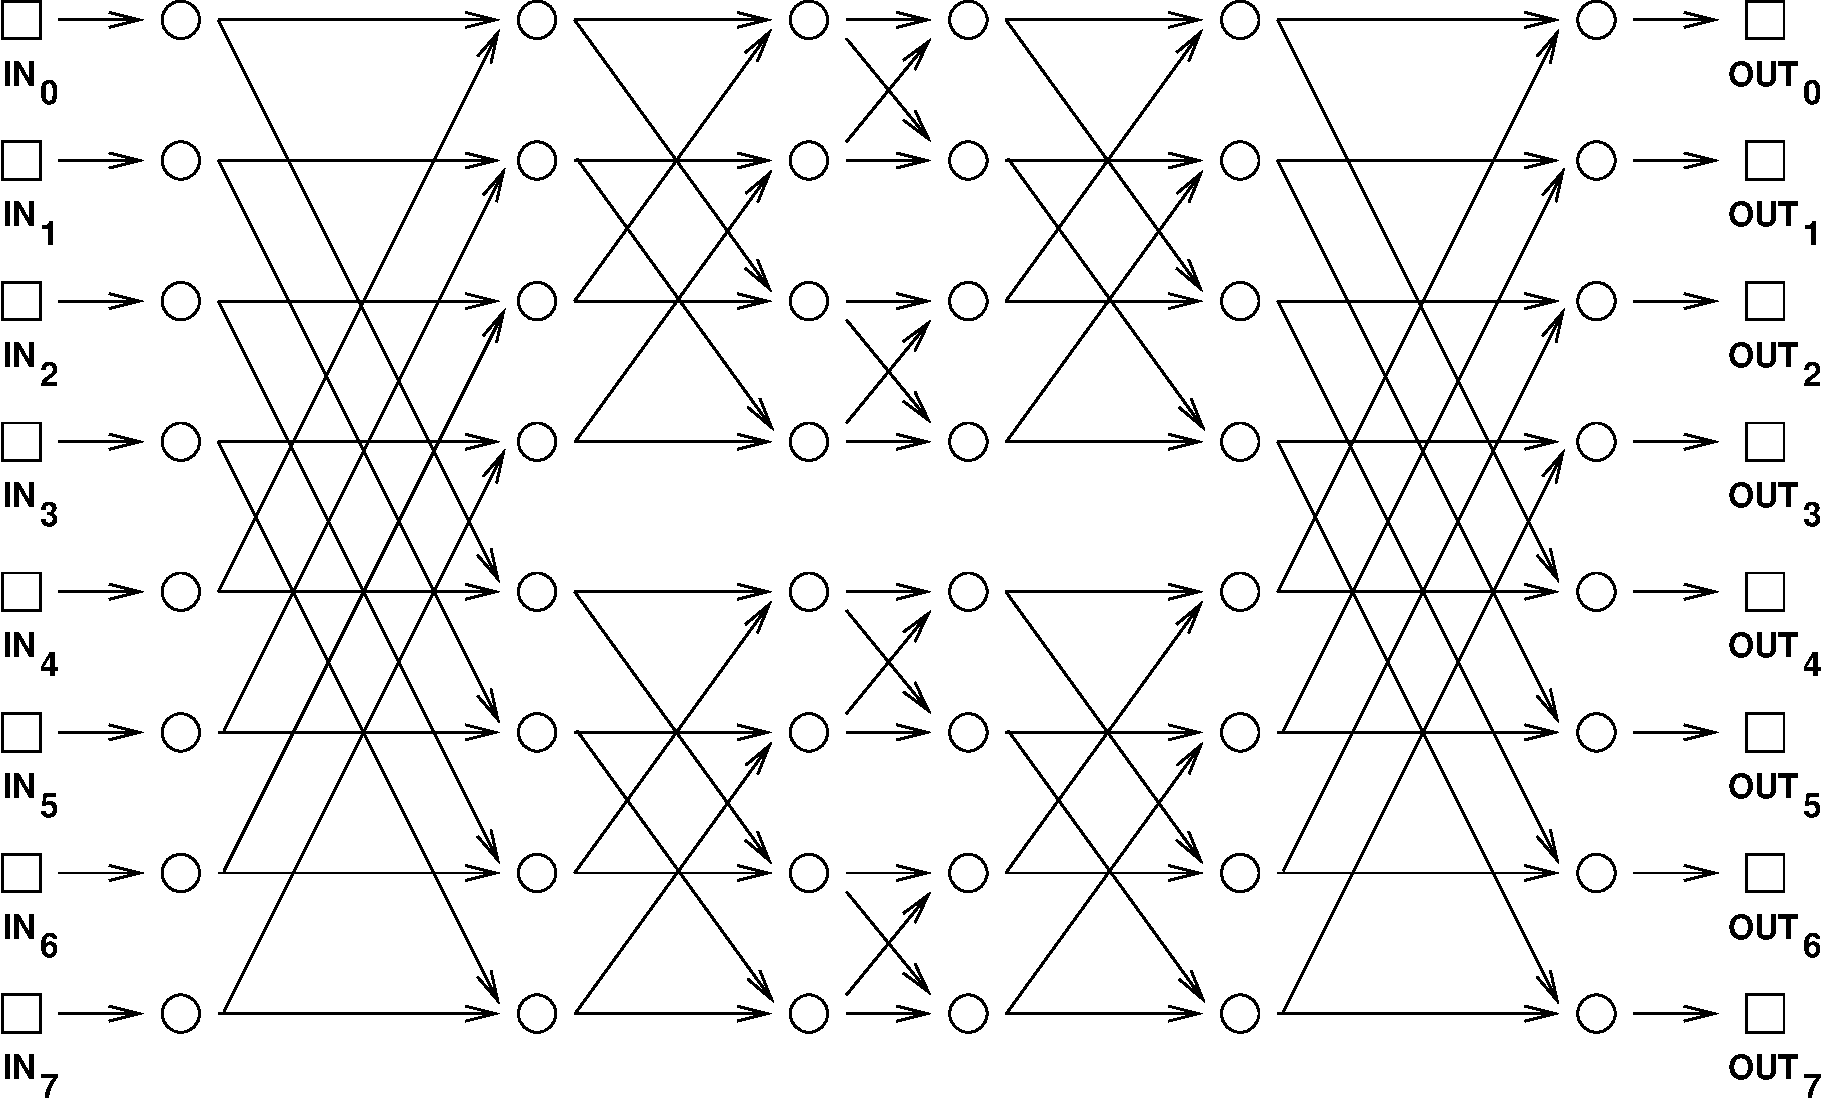
\includegraphics
[width=8.25in]{benes}}

%%%%%%%%%%%%%%%%%%%%%%%%%%%%%%%%%%%%%%%%%%%%%%%%%%%%%%%%%%%%%%%%%%%%%%%%%%%%%%%

\end{document}
